% !TeX root = ../../Book1.tex
% 纲要标题：### C.2 树作用与几何群论
% 纲要位置：计划纲要.md，第 897 行。
% BEGIN APPENDIX OUTLINE SYNC
% #### C.2.1 自由积的陪集树
% #### C.2.2 有限群作用的不动点
% #### C.2.3 字长与群的几何
% END APPENDIX OUTLINE SYNC

\section{树作用与几何群论}
\label{b1:sec:C02}

自由积的交替字可以用沿图行走来解释：相邻字母来自不同因子，对应路径不断向前而不立即沿原边退回。下面构造这样一个图，再用标准形证明它没有回路。

\ProseParagraphBreak
所用图由顶点、边及每条边的两个端点组成，边不指定方向。顶点的度是与它相接的边数；同时置换顶点和边、并保持端点关系的映射称为图自同构。一条路径记录依次经过的顶点与相邻边，其长度是边数；首尾顶点相同时，它是闭路径。若连续两步沿同一条边走过去再走回来，这两步构成回折，将它们删去就是消去回折。若路径的顶点不重复，称其为简单路径；长度为正、首尾相同、其余顶点不重复且不立即往返的闭路径称为回路。

\ProseParagraphBreak
树是连通而无回路的图，因此任意两顶点间恰有一条简单路径：连通性保证存在，若有两条不同的简单路径，取它们分开后重新相遇的部分，就得到回路。即使一棵树只有两个顶点 \(v,w\) 和连接它们的一条边，也能沿这条边走出闭路径 \(v\to w\to v\)；它只是一次回折，消去后得到长度零的路径，并不是回路。群在图上的作用，就是把每个群元素表示为一个图自同构，并要求这种表示保持群乘法。

\subsection{自由积的陪集树}
\label{b1:subsec:C02:01}

令 \(G=A*B\)。为把交替字解释为路径，我们希望右乘一个 \(A\) 中的字母时，前后的两条边在同一个 \(A\) 型顶点相接；右乘 \(B\) 中的字母时，则在 \(B\) 型顶点相接。右乘 \(A\) 中的元素恰好保持左陪集 \(gA\)，所以构造图 \(T\)：顶点集是不相交并 \(G/A\sqcup G/B\)，每个 \(g\in G\) 给出一条边，连接 \(gA\) 与 \(gB\)。这里 \(G/A\)、\(G/B\) 只是左陪集的集合，不要求因子正规，也没有赋予它们商群结构。即使两个因子抽象同构，也保留两种顶点类型，分别称为 \(A\) 型和 \(B\) 型。

\ProseParagraphBreak
这个定义同时记录了“哪些群元素相差一个因子元素”。编号为 \(g\) 与 \(g'\) 的两条边在一个 \(A\) 型顶点相接，当且仅当
\[
gA=g'A
\quad\Longleftrightarrow\quad
A=g^{-1}g'A
\quad\Longleftrightarrow\quad
g^{-1}g'\in A;
\]
\(B\) 型顶点相应记录 \(B\) 中的差别。群元素 \(h\) 的作用是把顶点 \(gA\)、\(gB\) 送到 \(hgA\)、\(hgB\)，把编号为 \(g\) 的边送到编号为 \(hg\) 的边。这些规则保持端点关系，并由群乘法的结合律给出群作用。

\begin{proposition}\label{b1:prop:free-product-coset-tree}
设 \(A,B\) 为群，\(G=A*B\)。令图 \(T\) 的顶点集为 \(G/A\sqcup G/B\)，并对每个 \(g\in G\) 设置一条连接 \(gA\) 与 \(gB\) 的边；\(G\) 以左乘作用在顶点和边上。则 \(T\) 是树，顶点 \(gA,gB\) 的稳定子群分别为 \(gAg^{-1},gBg^{-1}\)，每条边的稳定子群均为单位群。
\end{proposition}

\begin{proof}
边 \(g\) 与边 \(ga\)（\(a\in A\)）有公共端点 \(gA\)，边 \(g\) 与边 \(gb\)（\(b\in B\)）有公共端点 \(gB\)。给定 \(g=x_1\cdots x_n\) 的交替字，依次经过编号为
\[
1,\ x_1,\ x_1x_2,\ \ldots,\ x_1\cdots x_n=g
\]
的边：每次右乘 \(x_i\)，都经由其所属因子对应的顶点到达下一条边。这给出从单位边到边 \(g\) 的路径；又每个顶点都是某条边的端点，故图连通。

若有回路，按次序记边为 \(g_0,g_1,\ldots,g_{m-1},g_m=g_0\)，并令 \(x_i=g_{i-1}^{-1}g_i\)。相邻边在 \(A\) 型或 \(B\) 型顶点相交，故 \(x_i\) 属于相应因子；回路不立即沿原边退回，所以相邻边不同，从而 \(x_i\ne1\)。顶点类型沿回路交替，因此 \(x_1\cdots x_m\) 是非空约化字。另一方面，中间因子逐一抵消给出
\[
x_1\cdots x_m
=(g_0^{-1}g_1)(g_1^{-1}g_2)\cdots(g_{m-1}^{-1}g_m)
=g_0^{-1}g_m=1,
\]
与\cref{b1:lem:free-product-normal-form}的非空约化字非单位相矛盾。故图无回路。

等式 \(hgA=gA\) 当且仅当 \(g^{-1}hg\in A\)，给出第一个稳定子群公式；将 \(A\) 换成 \(B\) 得到第二个公式。边按群元素本身编号，\(hg=g\) 迫使 \(h=1\)，故边稳定子群平凡。
\end{proof}

取 \(A=C_2=\langle a\mid a^2=1\rangle\)、\(B=C_3=\langle b\mid b^3=1\rangle\)。在\cref{b1:fig:free-product-coset-tree}中，单位边连接 \(A\) 与 \(B\)；边 \(a\) 连接 \(A\) 与 \(aB\)，边 \(b,b^2\) 分别连接 \(B\) 与 \(bA,b^2A\)。一般地，与 \(gA\) 相接的边恰以 \(ga\) 为编号，其中 \(a\in A\)，所以 \(A\) 型顶点的度为二；\(B\) 型顶点的度为三。无限群 \(C_2*C_3\) 因而作用在局部有限的无限树上，这里的“局部有限”是指每个顶点的度都有限。

\begin{figure}[htbp]
\centering
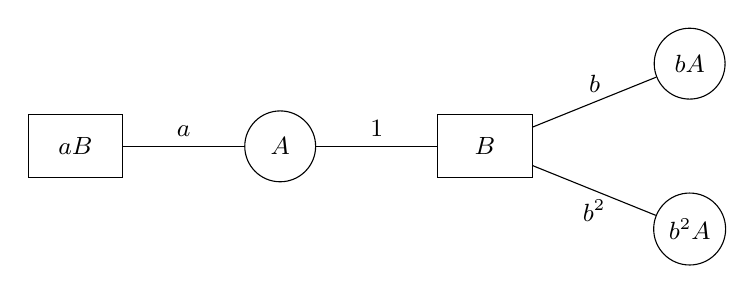
\begin{tikzpicture}[x=1cm,y=1cm,every node/.style={font=\small}]
\node[draw,rectangle,minimum width=12mm,minimum height=8mm] (aB) at (-4,0) {\(aB\)};
\node[draw,circle,minimum size=9mm] (A) at (-1.4,0) {\(A\)};
\node[draw,rectangle,minimum width=12mm,minimum height=8mm] (B) at (1.2,0) {\(B\)};
\node[draw,circle,minimum size=9mm] (bA) at (3.8,1.05) {\(bA\)};
\node[draw,circle,minimum size=9mm] (bbA) at (3.8,-1.05) {\(b^2A\)};
\draw (aB)--node[above] {\(a\)} (A);
\draw (A)--node[above] {\(1\)} (B);
\draw (B)--node[above] {\(b\)} (bA);
\draw (B)--node[below] {\(b^2\)} (bbA);
\end{tikzpicture}
\caption[自由积陪集树的局部]{\(C_2*C_3\) 陪集树中单位边附近的部分。圆形表示 \(A\) 型顶点，方形表示 \(B\) 型顶点；顶点标签是左陪集，边标签是群元素。边界处的顶点仍继续向外连接。}
\label{b1:fig:free-product-coset-tree}
\end{figure}

这棵陪集树与 \(G\) 的 Cayley 图不同。后者的顶点是群元素，左乘作用的顶点稳定子群平凡；前者的顶点是陪集，\(gA,gB\) 的稳定子群分别为 \(gAg^{-1},gBg^{-1}\)。因此，陪集树将因子及其共轭子群表示为顶点稳定子群，下一小节正会利用这一点研究自由积中的有限子群。例如 \(C_2*C_3\) 关于 \(\{a,b\}\) 的 Cayley 图中，关系 \(b^3=1\) 给出由 \(1,b,b^2\) 构成的三角形，陪集图却是树。一般的带合并自由积也有以 \(G/C\) 为边集的类似树；本附录不再展开这一推广的图论证明。

\subsection{有限群作用的不动点}
\label{b1:subsec:C02:02}

设群 \(G\) 作用在树 \(T\) 上。若不存在保持某条边却交换其两个端点的群元素，则称该作用\term[wu-fanzhuan-shuzuoyong]{无反转}[without inversions]。上面的陪集树作用保持顶点类型，因而无反转。若某个元素交换一条边的两个端点，在这条边中点加入一个顶点后，它会固定中点并交换两条新边，因而不会反转其中任何一条。对每条边都这样细分，并把原图自同构延拓到中点，就得到无反转作用：每条新边都有一个旧顶点和一个新中点，而群作用保持这两类顶点。

\begin{theorem}\label{b1:thm:finite-group-tree-fixed-point}
设有限群 \(G\) 以无反转方式作用在非空树 \(T\) 上。则 \(T\) 中存在被 \(G\) 的每个元素固定的顶点。
\end{theorem}

\begin{proof}
取顶点 \(v\)。因为 \(G\) 有限，其轨道 \(Gv\) 有限。若轨道只有一个顶点，\(v\) 已是公共不动顶点。否则将轨道中各对顶点之间的唯一简单路径取并，记为 \(T_0\)。轨道只有有限多对顶点，每条路径又只有有限条边，故并集是有限图；它连通且位于树中，因而是有限子树。图自同构把唯一简单路径送到相应端点间的唯一路径，且置换 \(Gv\)，所以保持 \(T_0\)。

在有限树中，度为一的顶点称为叶顶点。我们要在 \(T_0\) 中找到一个由树本身确定、被所有图自同构保持的顶点或边；同时反复削去全部叶顶点，便会留下这样的中心。若 \(T_0\) 多于两个顶点，同时删掉全部叶顶点及所连边。剩余图非空：最长简单路径至少有两条边，它的内点不会在这一步被删去。剩余图也仍连通，因为两保留顶点之间的路径不可能以内点为叶顶点。它仍是树，并被 \(G\) 保持，因为图自同构保留各顶点的度，从而置换整批叶顶点。有限树的最长简单路径两端都是叶顶点，否则还能向外延长；故只要还多于两个顶点，删除就严格减少顶点数。反复操作最终剩下一个顶点或一条边。前者就是公共不动顶点；后者被全群保持，无反转条件使每个群元素都固定其两个端点。
\end{proof}

\begin{corollary}\label{b1:cor:finite-subgroup-free-product}
设 \(A,B\) 为群。自由积 \(A*B\) 的任意有限子群都包含于 \(A\) 或 \(B\) 的某个共轭子群中。
\end{corollary}

\begin{proof}
设 \(H\le A*B\) 是有限子群，将陪集树上的作用限制到 \(H\)。这个作用保持两类顶点，因而无反转；由\cref{b1:thm:finite-group-tree-fixed-point}，\(H\) 固定某个 \(gA\) 或 \(gB\)。在前一种情形，
\[
H\le\operatorname{Stab}(gA)=gAg^{-1},
\qquad g^{-1}Hg\le A;
\]
后一种情形同样得到 \(g^{-1}Hg\le B\)。
\end{proof}

特别地，\(C_2*C_3\) 中有限阶元素的阶只能是 \(1,2,3\)。这给出了上一节无限阶计算的结构性解释。

\ProseParagraphBreak
结论中的“公共”十分重要：要找到的是同一个被群中每个元素固定的顶点。上述证明先取整个轨道，再同时删去全部叶顶点，正是为了使每一步留下的子树都被全群保持，而不必分别为各群元素寻找顶点。

\subsection{字长与群的几何}
\label{b1:subsec:C02:03}

设群 \(G\) 由非空有限集 \(S\) 生成。对 \(g\in G\)，令 \(\ell_S(g)\) 为用 \(S\cup S^{-1}\) 表示 \(g\) 所需的最少字母数，其中单位元允许用长度零的空字表示。由于 \(S\) 生成 \(G\)，候选长度组成一个非空的非负整数集合，最小值因而存在。称 \(\ell_S(g)\) 为 \(g\) 关于 \(S\) 的\term[zi-chang]{字长}[word length]。再令
\[
d_S(g,h)=\ell_S(g^{-1}h).
\]
这是一个左平移不变的距离，因为对任意 \(k\in G\)，
\[
d_S(kg,kh)=\ell_S((kg)^{-1}kh)=\ell_S(g^{-1}h)=d_S(g,h).
\]
右平移却给出 \(d_S(gk,hk)=\ell_S(k^{-1}g^{-1}hk)\)，字长一般不会在共轭下保持，所以不必右平移不变。例如在自由群 \(F(a,b)\) 中取 \(S=\{a,b\}\)，有 \(d_S(1,a)=1\)，右乘 \(b\) 后却有 \(d_S(b,ab)=\ell_S(b^{-1}ab)=3\)。非负性和零距离判据直接来自定义，逆字说明对称性，而串接给出 \(\ell_S(xy)\leq\ell_S(x)+\ell_S(y)\)，从而有三角不等式。它就是第八章所述 Cayley 图的边路径距离，见\subsecref{b1:subsec:0804:03}。
\symidx{\(\ell_S(g),d_S(g,h)\)：生成集 \(S\) 所定的字长与字距离}

\ProseParagraphBreak
例如加法群 \(\mathbb Z\) 对生成集 \(\{1\}\) 有 \(\ell(n)=|n|\)、\(d(m,n)=|n-m|\)。对于 \(\mathbb Z^2\) 的生成集 \(\{(1,0),(0,1)\}\)，每步只能把一个坐标改变一，所以到达 \((m,n)\) 至少需要 \(|m|+|n|\) 步；先沿第一坐标再沿第二坐标行走就达到此界。因此字长为 \(|m|+|n|\)，对应方格图中的最短路径长度。

\ProseParagraphBreak
字长依赖生成集，但有限生成集之间的变化受到统一控制。若 \(S,T\) 都非空、有限且生成 \(G\)，令
\[
M=\max\bigl(1,\max_{s\in S}\ell_T(s)\bigr),\qquad
N=\max\bigl(1,\max_{t\in T}\ell_S(t)\bigr).
\]
把最短 \(S\)-字中的每个字母换成长度至多 \(M\) 的 \(T\)-字，就得到 \(d_T(g,h)\leq M d_S(g,h)\)；逆字母的替换长度也相同。交换 \(S,T\) 给出 \(d_S(g,h)\leq N d_T(g,h)\)，所以对所有 \(g,h\in G\)，
\[
\frac{1}{N}d_S(g,h)\leq d_T(g,h)\leq M d_S(g,h).
\]
两个字距离相互控制在固定倍数以内，但这种比较不要求图的局部结构相同。例如，在自由群 \(F(a,b)\) 中给自由基 \(\{a,b\}\) 增添冗余生成元 \(ab\)，新的 Cayley 图便出现由 \(1,a,ab\) 构成的三角形；新增的边改变了局部路径，却没有破坏上述距离界。

\ProseParagraphBreak
\term[jihe-qunlun]{几何群论}[geometric group theory]利用这种距离和群作用研究群。例如自由群相对于一组自由基的 Cayley 图是树，而 \(\mathbb Z^2\) 对标准生成集的 Cayley 图是有许多四边形的方格图。路径是否容易约化、球中元素数怎样增长、子群怎样作用于空间，都是把代数问题转成几何问题的方式。本附录只建立树这一模型；曲率、双曲群与更一般的几何方法需要另外的准备。
